\documentclass{beamer}
\mode<presentation>
\usepackage{amsmath}
\usepackage{amssymb}
\usepackage{bm}		
\usepackage{color}
\usepackage{hyperref}
\usepackage{graphicx,color}
\usepackage[ngerman]{babel}
\usepackage{color}
\usepackage{float}
\usepackage{graphicx}
\usepackage{graphicx,color}
\usepackage{scrextend}
\usepackage{subfigure}
\usepackage{tabularx}
\usepackage{fancyhdr}
\usepackage{graphicx}
\usepackage{etoolbox}
\usepackage{graphicx}
\usepackage{titlesec}
\usepackage{caption}
\usepackage{booktabs}
\usepackage{xcolor}
\usepackage{caption}
\usepackage{float}
\captionsetup[figure]{name=Figure}
\usepackage{setspace}
\def\plim{\mathop{\rm plim}\limits}
\def\argmin{\mathop{\rm argmin}\limits}
\def\argmax{\mathop{\rm argmax}\limits}
\def\ln{\mathop{\hbox{ln }}}
\def\E{\mathop{\mathbb{E}}\limits}
\newcommand{\Perp}{\perp \! \! \! \! \perp}

\definecolor{light-gray}{gray}{0.92}
\newcommand{\blue}[1]{\textcolor{blue}{#1}}
\newcommand{\red}[1]{\textcolor{red}{#1}}
\newcommand{\white}[1]{\textcolor{white}{#1}}\makeatletter

\setbeamertemplate{footline}[frame number]
\def\plim{\mathop{\rm plim}\limits}
\def\argmin{\mathop{\rm argmin}\limits}
\definecolor{rosa}{rgb}{1,0.2,0.5}
\title{\bf Optimal estimators for synthetic controls}\vspace{1cm}

\author{{{ J\"org Breitung}, Lennart Bolwin  and Justus T\"ons \\[2mm] \textit{University of Cologne }}}

\date[]{ \textcolor{brown}{Goethe-University Frankfurt, June 23rd, 2023 }}
%\usetheme{Bergen}



\begin{document}
\begin{frame}
  \titlepage
\end{frame}
% =========================== Page 3 ====================== @

\begin{frame}{\bf Background}
\begin{itemize}
\item potential outcome framework developed by Neyman (1923) and refined by Rubin (1974).

\item Let $Y^{I}_{0,t}$ be the (potential) outcome for the treated unit $i=0$ in $t$
\item and $Y^{N}_{i,t}$ is the (potential) outcome for in the \alert{absence} of the intervention.

\item treatment effect is defined as
\[
\delta_{t} = Y^{I}_{0,t} - Y^{N}_{0,t}
\]
%and define the treatment dummy as $D_{t}$ with $D_t=1$ if the treatment applies in $t$.

\item Accordingly
\[
Y_{j,t}^I = \begin{cases}
	Y^{N}_{0,t} &\text{for }  t \le T_0   \\
	Y^{N}_{0,t} + \red{\delta_{t} } &  \text{for  } t > T_0
\end{cases}
\]
\item goal: estimate the causal treatment effect $(\delta_{T_0}, ..., \delta_{T})$  \newline
\red{counterfactual:} {\it trajectory if there was no intervention}
\end{itemize}
\end{frame}

\begin{frame}{\bf Abadie/Diamond/Hainmueller (2003) approach}
\begin{itemize}
\item Assume that there exist $n$ additional \blue{untreated} time series $Y_{1,t},\ldots,Y_{n,t}$ for $t=1,\ldots,T_0,\ldots,T$
\item ADH assume that the counterfactual can be approximated by
\begin{align*}
\widehat Y^{N}_{0,t} &\approx \sum_{i=1}^n \red{w_{i,t}} Y_{j,t}
\end{align*}
\item The weights are determined in an additional step by using vectors of $k$ \blue{time independent} \red{pre-treatment} variables $\bm{x}_0,\bm{x}_1,\ldots,\bm{x}_n$
\item The weights are obtained from minimizing the criterion function
\begin{align*}
\widehat{\bm w}(\bm{v}) &= \argmin_{\bm{w}} \left\{ \sum_{j=1}^k v_j \left( x_{0,j} - \sum_{i=1}^n w_i x_{i,j}\right)^2 \right\}
\end{align*}
under the (regularisation) constraints:
\begin{align*}
 \red{ \text{ no constant} } \quad
 \blue{ 0 < w_i < 1 \quad
 \sum_{i=1}^n w_i = 1 }
\end{align*}
\end{itemize}
\end{frame}

\frame{

\begin{center}

Example: German reunification

 \includegraphics[width=1.00\textwidth]{Fig1_Abadie.pdf} \vspace{-0.8cm}

 \includegraphics[width=1.00\textwidth]{Tab1_Abadie.pdf}
\end{center}
}

\frame{

 \includegraphics[width=1.00\textwidth]{Tab2_Abadie.pdf}

}

\begin{frame}{Critique}

\begin{itemize}
\item a sound statistical framework is missing (only a rudimentary framework is provided based on a static factor model)
\item the relationship between $Y$ and $\bm{x}$ is not clear
\item Consistency for $T_0\to \infty$ and $n\to \infty$ and $n/T_0\to 0$?
\item Optimal estimator for the counterfactual?
\item Leaving out the constant and the restrictions on $w_i$ may result in \red{biased} estimates
\item How to choose $\bm(v)$?
\item How is this approach related to the standard treatment-effect models?
\item Some of these concerns are already raised in Doudchenko and Imbens (2017)
\end{itemize}
\end{frame}

\begin{frame}{Relationship to the traditional literature on treatment-effect}

\begin{itemize}
\item we follow to some extend Doudchenko and Imbens (2017)
\item A natural estimator is the \blue{DiD}-estimator that yields for $\tau>T_0$
\begin{align*}
\widehat \delta_\tau^{did} &= \underbrace{ \red{Y_{0,\tau}} \blue{- \widehat \mu_0^0}}_{\text{a-b treated}} \ - \ \underbrace{ \red{ \sum_{i=1}^n \left( \frac{1}{n} \right) Y_{i,\tau} } \blue{ - \frac{1}{n} \sum_{i=1}^n \left( \widehat \mu_i^0\right)} }_{\text{a-b control}}
\end{align*}
where $\widehat \mu_i^0$ denote the pre-treatment sample mean of the series \smallskip

\item This estimator is somehow \blue{related to the ADH-approach}: \smallskip

\begin{itemize}
\item the weights are given by $1/n$
\item no $\bm{x}_i$ is required as the weights are fixed in advance
\item The estimate are corrected for the different means of the series (in contrast to ADH)
\end{itemize}
\end{itemize}
\end{frame}

\begin{frame}{\bf Optimal synthetic controls: the static case}

\begin{itemize}
\item What is the optimal estimator of $\delta$ if we assume that
\[
\boldsymbol{y} = \begin{pmatrix} Y_0 \\ Y_1\\ Y_2 \end{pmatrix} \ \stackrel{iid}{\sim} \ \mathcal{N}(\boldsymbol{\mu},\boldsymbol{\Sigma})
\text{ before } T_0
\]
where $\boldsymbol{\mu} = \left(\mu_0, \mu_1, \mu_2  \right)^\prime$ and $\boldsymbol{\Sigma}\begin{pmatrix} \sigma_0^2 & \boldsymbol{\sigma}_{21}' \\ \boldsymbol{\sigma}_{21} & \boldsymbol{\Sigma}_2 \end{pmatrix}$
\item Assuming that the distribution is known, the UMV estimator is given by
{\small \begin{align*}
\widehat \delta &=  Y_0^I - \E(Y_0^N|Y_1,Y_2) \\
\E(Y_0^N|Y_1,Y_2)  &= \mu^* + \red{w_1} Y_1 + \red{w_2} Y_2
\end{align*} }
where $\mu^*=\mu_0 - w_1\mu_1 - w_2\mu_2$ and
\begin{align*}
\begin{pmatrix} w_1 \\ w_2 \end{pmatrix} &= \boldsymbol{\Sigma}_2^{-1} \boldsymbol{\sigma}_{21}
\end{align*}
\item The estimator for the CF is \red{consistent} if \blue{$n/T_0 \to 0$}
\end{itemize}
\end{frame}

\begin{frame}{Comments}

\begin{itemize}

\item solution is similar to \red{DiD-estimator} but with \blue{different weights}
\item the weights depend on the correlation among the $Y_i$
\item the \red{DiD}-estimator assumes that $Y_i$ are equi-correlated (``time effect'') and under this assumption the estimator is identical
\item the optimal estimator does not impose the ADH-restrictions:
\begin{itemize}
\item the constant is different from zero in general
\item the weights do not need to be positive
\item the weights do not add-up to one
\end{itemize}
\item For illustration assume that
{\footnotesize \begin{align*}
y &\sim {\cal N}\left( \begin{pmatrix} 1 \\ 1 \\ 1 \end{pmatrix}, \begin{pmatrix} 1 &  0.1 & 0.4 \\ 0.1 & 1 & 0.5 \\ 0.4 & 0.5 & 1 \end{pmatrix} \right)
\end{align*} }
optimal weights: \red{$w_1=-0.133$}, \blue{$w_2=0.4667$}.
\item ADH is \red{biased} if $\mu_i$ differ and var(AHD) =1.16 compared to var(optimal) =  0.827
\end{itemize}
\end{frame}

\begin{frame}{\bf Estimation}
\begin{itemize}
\item so far we assumed that the joint distribution of $Y_1,\ldots,Y_n$ is known
\item OLS (plug-in) estimator:
{\small \begin{align*}
Y_{0,t} = \mu^* + \sum_{i=1}^n \blue{w_i} Y_{i,t} + u_i  \ \text{ for } \ t=1,\ldots,T_0
\end{align*} }
\item poor small sample properties if $n/T_0$ is substantial (say $> 0.2$)
\item regularized (shrinkage) estimator minimizes
{\footnotesize \begin{align*}
Q(w,\lambda_1,\lambda_2) &= \sum_{t=1}^{T_0} \left( y_{0t}- \mu^* - \sum_{i=1}^n w_i y_{it}\right)^2  + \blue{\lambda_1 \left( \sum_{i=1}^n w_i^2 \right)} + \red{\lambda_2 \left(1- \sum_{i=1}^n  w_i\right)^2}
\end{align*}}
\begin{itemize}
\item the blue penalty term is the usual Ridge penalty
\item the red term favors weights adding up close to one
\item if $\lambda_1$ and $\lambda_2$ get large $w_i \to 1/n$
\item the minimum of $Q$ given $\lambda_1$ and $\lambda_2$ has an explicit solution
\item similar but simpler and more natural than elastic net of DI
\end{itemize}
\end{itemize}
\end{frame}

\begin{frame}{\bf Factor models}

\begin{itemize}
\item original ADH approach was motivated by a factor model
\item ADH (2010) assume a perfect control with \red{$Y_{0,t}=\sum_i w_i Y_{i,t}$}
\item let us assume a factor model:
{\small \begin{align*}
Y_{i,t} &= \mu_i + \lambda_{1i} \red{f_{1,t}} + \ldots + \lambda_{ri} \red{f_{r,t}}  + \epsilon_{i,t}
\end{align*}}
\item the \blue{optimal estimator} for the synthetic control is ($r=1$)
{\small \begin{align*}
\widehat Y_{0t}^N &=  \E( Y_{0t}| Y_{1,t},\ldots,Y_{n,t} ) \quad \textcolor{brown}{ \text{ for } t=1,2,\ldots, T_0 } \\
&= \mu_0 + \lambda_0 \, \blue{ \E( f_{t}| Y_{1,t},\ldots,Y_{n,t} )}
\end{align*} }
\item this suggest the following \red{plug-in estimator}:
\begin{enumerate}
\item estimate the common factor(s) among $Y_{1,t},\ldots,Y_{n,t}$ for $t=1,\ldots,T_0$ by PCA
\item run a regression of $Y_{0,t}$ on $(\widehat f_{1,t},\ldots,\widehat f_{r,t})$ and a constant and denote the fitted values by $\widehat Y_{0,t}$
\item run a regression $\widehat Y_{0,t}$ on $Y_{1,t},\ldots,Y_{n,t}$ and a constant. The coefficients are the estimated weights
\end{enumerate}
\item resulting estimator is another regularized estimator where a factor structure is imposed to CovMat
\end{itemize}
\end{frame}


\begin{frame}{\bf Monte Carlo simulations}

\begin{itemize}
\item Following Ferman (2021) we consider a factor model with $Y_{i,t}^{N} = \mu_i + \lambda_i'f_t + \epsilon_{i,t}$ with \red{$r=2$ factors}
\item The first and second factor loads on the treated unit and the first/second half of the donor pool.
\item The loadings are all equal to one
\item We simulate a total of $T_0$ pre-treatment and $T_1$ post-treatment observations
\item Size of the donor pool: $n \in \left\lbrace 5,10,20,30\right\rbrace$.
\item $\mu_i$, $f_{1t}$, $f_{2t}$ and $\epsilon_{it}$ are \textit{iiN}(0,1) \smallskip

{\footnotesize \begin{itemize}
\item {\bf FACTOR}: PCA-estimator based on the factor model
\item {\bf SC}: Synthetic-Control-Model of ADH (2010)
\item {\bf REGOLS}: regularized OLS regression equal weight penalty
\item {\bf NET}: regularized OLS regression with Elastic Net proposed by Doudchenko and Imbens (2017)
\item {\bf OLS}: OLS estimator without penalty
\end{itemize} }
\end{itemize}
\end{frame}

\frame{
{\small
\begin{table}[H]
	\centering
	\noindent
	\caption{Static Factor Model with \textbf{J = 10} Donors.}
	\scalebox{1}{
		\begin{tabular}{c c | c | c | c | c | c }
			\toprule[1.5pt]
			\multicolumn{1}{c}{$\boldsymbol{T_0}$} & \multicolumn{1}{c}{$\boldsymbol{T_1}$}& \multicolumn{1}{c}{\textbf{FACTOR}} & \multicolumn{1}{c}{\textbf{SC}} & \multicolumn{1}{c}{\textbf{REGOLS}}& \multicolumn{1}{c}{\textbf{NET}}& \multicolumn{1}{c}{\textbf{OLS}}\\
			\cmidrule(lr){1-7}
			& & RMSE&RMSE&RMSE&RMSE&RMSE\\
			\cmidrule(lr){1-7}
			20&30&1.1613&1.2867&1.2304&1.2739&1.6198\\
			&20&1.1555&1.2840&1.2250&1.2595&1.6167\\
			&10&1.1312&1.2532&1.1987&1.2395&1.5811\\
			\cmidrule(lr){1-7}
			% next specification
			50&30&1.1043&1.2497&1.1369&1.1467&1.2086\\
			&20&1.0966&1.2308&1.1317&1.1407&1.2074\\
			&10&1.0912&1.2167&1.1204&1.1281&1.1895\\
			\cmidrule(lr){1-7}
			% next specification
			100&30&1.0851&1.2316&1.1063&1.1112&1.1323\\
			&20&1.0733&1.2088&1.0917&1.0941&1.1202\\
			&10&1.0661&1.1986&1.0895&1.0934&1.1178\\
			\bottomrule[1.5pt]
	\end{tabular}}
\end{table}}
}

\frame{
{\small \begin{table}[H]
	\centering
	\noindent
	\caption{Static Factor Model with \textbf{J = 30} Donors.}
	\scalebox{1}{
				\begin{tabular}{c c | c | c | c | c | c }
			\toprule[1.5pt]
			\multicolumn{1}{c}{$\boldsymbol{T_0}$} & \multicolumn{1}{c}{$\boldsymbol{T_1}$}& \multicolumn{1}{c}{\textbf{FACTOR}} & \multicolumn{1}{c}{\textbf{SC}} & \multicolumn{1}{c}{\textbf{REGOLS}}& \multicolumn{1}{c}{\textbf{NET}}& \multicolumn{1}{c}{\textbf{OLS}}\\
			\cmidrule(lr){1-7}
			& & RMSE&RMSE&RMSE&RMSE&RMSE\\
			\cmidrule(lr){1-7}
			20&30&1.1013&NA&1.1899&1.2523&NA\\
			&20&1.1043&NA&1.1825&1.2442&NA\\
			&10&1.0890&NA&1.1647&1.2337&NA\\
			\cmidrule(lr){1-7}
			% next specification
			50&30&1.0622&1.1477&1.1039&1.1297&1.6851\\
			&20&1.0508&1.1372&1.0936&1.1190&1.6716\\
			&10&1.0445&1.1342&1.0880&1.1061&1.6681\\
			\cmidrule(lr){1-7}
			% next specification
			100&30&1.0420&1.1178&1.0662&1.0793&1.2394\\
			&20&1.0435&1.1237&1.0669&1.0788&1.2351\\
			&10&1.0159&1.0890&1.0410&1.0465&1.2026\\
			\bottomrule[1.5pt]
	\end{tabular}}
	\label{table:table S.6}
\end{table} }}


\frame{ \begin{figure}[H]
	\centering
    \vspace{-3.5cm}
	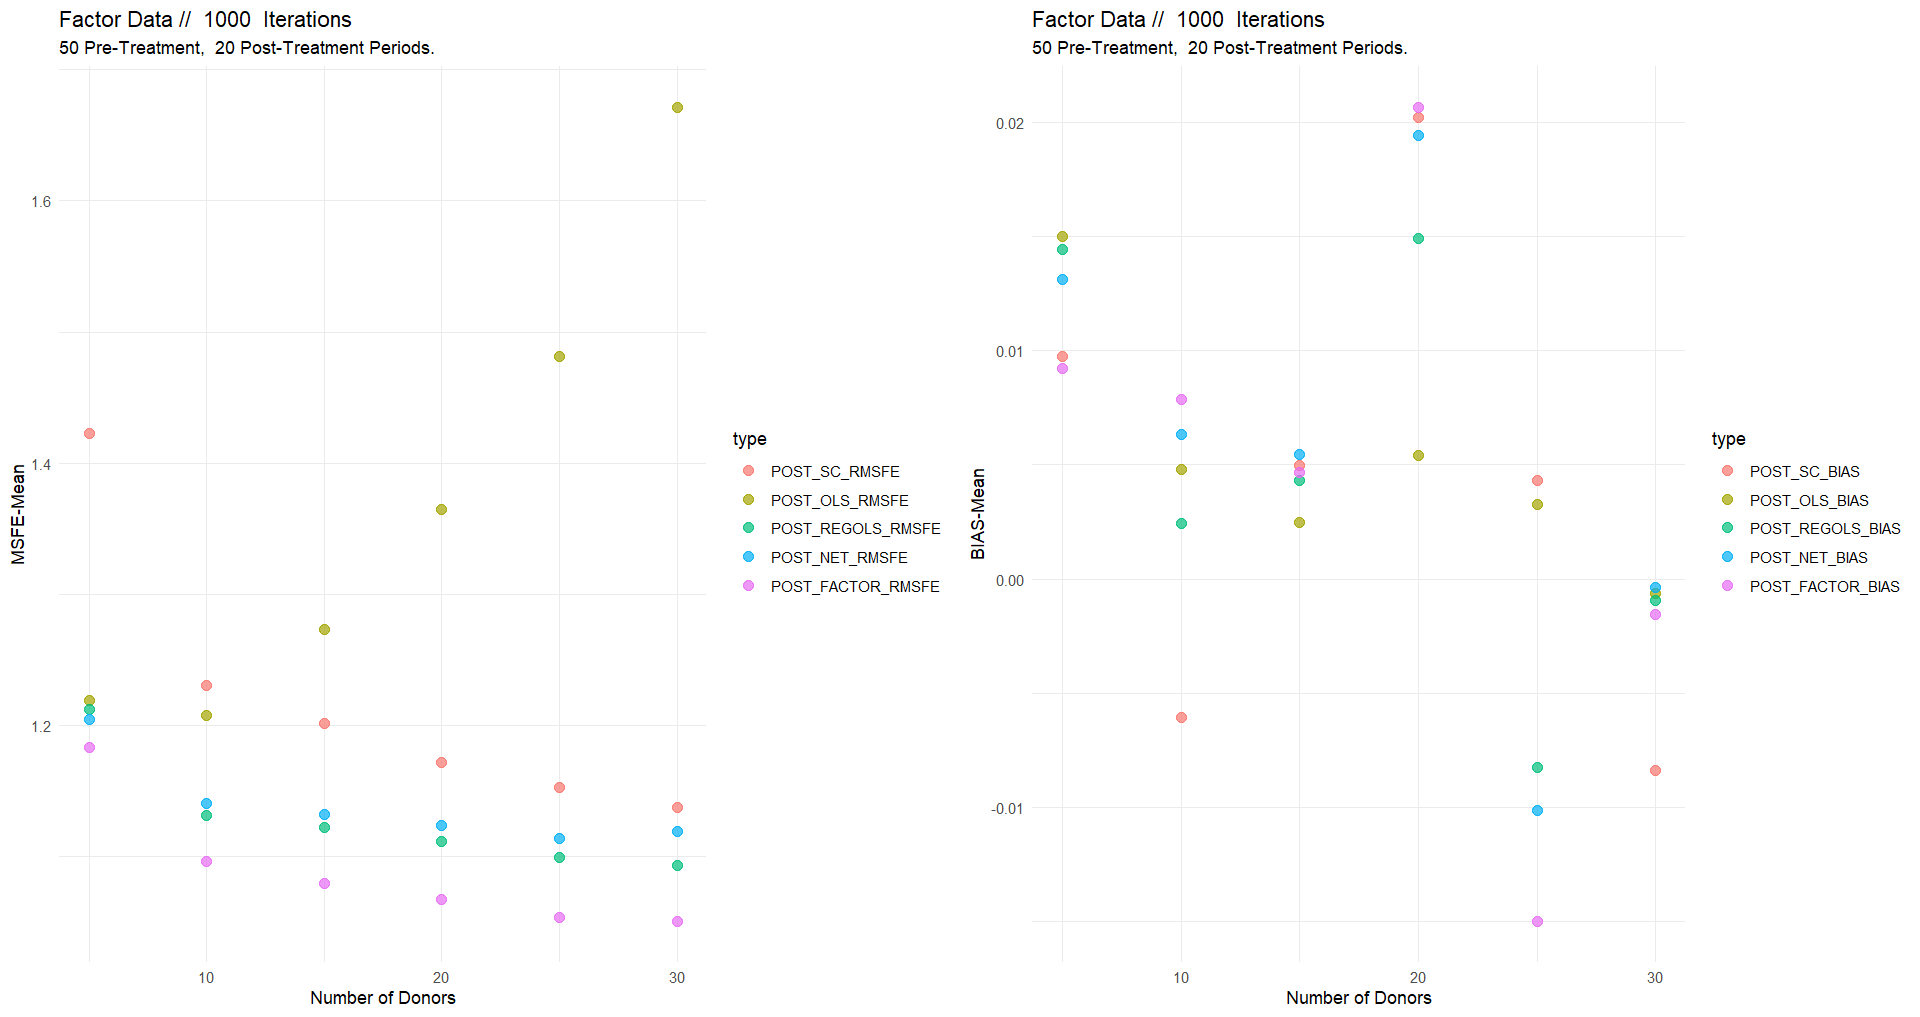
\includegraphics[scale=0.58]{05_Plot_50_20.png}
	\caption{Example Factor DGP}
\end{figure} }

\begin{frame}{\bf Dynamic models}

\begin{itemize}
\item Assume that the $(k+1) \times 1$ vector of time series $\bm{y}_t=(Y_{0,t},\ldots,Y_{n,t})'$ can be represented as
{\small \begin{align*}
\bm{y}_t &= \bm{\alpha} + \bm{A}_1 \bm{y}_{t-1} + \cdots + \bm{A}_p \bm{y}_{t-p} + \bm{u}_t \\
\bm{y}_t &= \bm{\mu} + \bm{A}(L)(\bm{y}_{t-1}-\bm{\mu}) + \bm{u}_t
\end{align*} }
where $\bm{\mu}=(\mu_0,\mu_1,\ldots,\mu_n)'$, $\E(\bm{u}_t \bm{u}_t')=\bm{\Sigma}$ is a positive definite covariance matrix.
\item The \blue{counterfactual} is given by
{\small \begin{align*}
\widehat Y_{0,t}^N &= \E( Y_{0,t}^N|{\cal I}_t ) \notag \\
&= \mu_0 + \sum_{i=1}^n w_i (Y_{i,t}-\mu_i) + \beta(L)'(\red{\widetilde y_{t-1}}-\mu)
\end{align*} }
where $\widetilde y_{t-1}-\mu) =(\red{\widehat Y_{0,t}^N} -\mu_0,Y_{1,t}-\mu_1,\ldots,Y_{n,t}-\mu_n)'$
\item lags of the series enter the estimated counterfactual
\item $\widehat Y_{0,t}^N$ needs to be estimated recursively
\end{itemize}
\end{frame}

\begin{frame}{\bf A univariate representation}

\begin{itemize}
\item using $\widehat Y_{0,t}^N = \bm{w}'\bm{y}_t$ we obtain the univariate representation:
{\small \begin{align}
\bm{y}_{0,t}^N &= \alpha_0 + \sum_{j=0}^p \alpha_j \left( \blue{ \bm{w}'\bm{y}_{t-j}} \right) + e_t \label{uni}
\end{align} }
\item estimate the parameters by sequential OLS:
\begin{itemize}
\item select some initial guess for $\bm{w}$ and estimate $\alpha_j$ in \eqref{uni} by OLS
\item fix $\alpha_j$ and estimate $\bm{w}$ by running the regression
{\small \begin{align*}
\bm{y}_{0,t}^N &= \alpha_0 + \bm{w}' \underbrace{ \left(  \sum_{j=0}^p \widehat \alpha_j \bm{y}_{t-j} \right)}_{ \mathbf{z}_t }  + e_t
\end{align*} }
 which yields the updated weights
\item repeat the estimation until convergence
\end{itemize}
\item Alternatively some regularized estimator for the full dynamic model may be used.
\end{itemize}
\end{frame}

\begin{frame}{\bf Conclusions}

\begin{itemize}
\item Synthetic control methods may be useful for assessing the \alert{causal} effect of economic interventions
\item if the \blue{donor series} are correlated with the treated series, then the weights are different from $(1/n)$ and needs to be estimated
\item we derive the optimal (OLS) estimator for the counterfactual in a simple static setup
\item we argue that the weights do not need to satisfy the adding-up constraint, not do they need to be positive
\item it is important to include a constant term when estimating the weights
\item if $n/T_0$ is substantial, some regularization is required
\item we propose some penalization that shrinks the estimates towards $1/n$
\item for dynamic model the optimal counterfactual involves the lags of the donor series
\item we propose a simple univariate autoregressive representation for the counterfactual
\end{itemize}
\end{frame}
\end{document}

